\chapter{Konzeption des verteilten Entwicklungssystems}\label{chap:konzeption}
\minitoc
In diesem Kapitel soll das Entwicklungssystem konzipiert werden.

Hierfür muss anfänglich ein grundsätzliches Entwicklungskonzept festgelegt
werden. Aus diesem Konzept ergeben sich dann die Voraussetzungen, die die zu
wählende Hardware erfüllen muss.

Das Entwicklungssystem soll außerdem dazu verwendet werden, ein
beispielhaftes Zielsystem entwickeln zu können. Auch über die Hardware dieses
Zielsystems muss eine Entscheidung getroffen werden, die möglichst
repräsentativ für eine Vielzahl möglicher Zielsysteme ist.

Letztendlich muss sichergestellt werden, dass alle einzelnen Komponenten in dem
zu planenden System miteinander interagieren. Es müssen
Schnittstellenspezifikationen festgelegt werden.
\section{Grundlegende Konzeption}
\begin{figure}[!ht]
\centering
\def\svgwidth{0.88\columnwidth}
\input{res/system.pdf_tex}\\
\caption{Das geplante Gesamtsystem}{Die "'Module"' werden über WLAN
vom Entwicklersystem gesteuert und übermitteln an dieses auch alle
Daten, die sie von ihrem jeweils angeschlossenen "`Ziel"' erhalten.}
\label{fig:sys}
\end{figure}
Der Umstand, dass die einzelnen Zielsysteme räumlich von einander und dem
Entwicklersystem getrennt sind, erfordert gewisse Änderungen an den
Entwicklungsabläufen.

Ein direkter Zugriff auf die einzelnen Zielsysteme ist nicht ohne Weiteres
möglich beziehungsweise vergleichsweise umständlich. Würde man die in
\autoref{chap:analyse} aufgezählten Abläufe für ein verteiltes System umsetzen
wollen, müsste man die Zielsysteme zum Beispiel neben das Entwicklersystem
legen, da für viele Vorgänge eine \textbf{physische Verbindung} bestehen muss.

So benötigt zum Beispiel das Debugging über \gls{jtag} oder \gls{swd} eine
Verbindung zwischen einem Adapter und dem Zielsystem sowie zwischen
Entwicklersystem und Adapter. Sollen beliebige Daten vom Zielsystem erfasst
werden, so wird auch hierfür oft eine Verbindung in Form von direkter
Verkabelung benötigt.

Die Auswahl existierender Netzwerk-Debugging-Lösungen ist geradezu
minimal. Als eigenständige Lösung findet sich hier zum Beispiel \emph{ZY1000
(Ultimate Solutions Inc.)}\cite{ULT} oder \emph{WiFiDemon (Macraigor
Systems)}\cite{MAC}. Beide Systeme stellen eine Schnittstelle zwischen Ethernet
oder WLAN dar und sind somit bereits existierende Teilumsetzungen des geplanten
\emph{Entwicklungssystems}.

Beide Lösungen sind jedoch auch geschlossene Systeme. Wollte man also, wie
vorgesehen, zusätzliche Daten sammeln, müsste man ein weiteres Gerät (mit
eigenem Anschluss an das Netzwerk) verwenden.

Der Ansatz vom in \autoref{sec:exist} erwähnten \emph{TinyOS}, das Funknetzwerk
der Zielsysteme selbst für das Deployment von Firmware oder das Analysieren von
internen Vorgängen zu nutzen, hat den Nachteil, dass dafür ein solches Netzwerk
bereits bestehen muss. Dies kann jedoch nicht immer garantiert werden.
Insbesondere nicht dann, wenn erwähntes Funknetzwerk erst noch entwickelt werden
muss.

Wünschenswert wäre es also, ein von dem Zielsystem und dessen Hardware völlig
unabhängiges System zu entwickeln. Dies hat gleichzeitig den Vorteil, dass es
bezüglich der Entscheidungen über ein Zielsystem \textbf{größtmögliche
Flexibilität} bietet.

Der Grundgedanke hinter dem zu entwerfenden Entwicklungssystem ist
deshalb der, dass bereits bestehende Infrastruktur wie Ethernet oder WLAN für
die Verbindung von "`Modulen"' zum Entwicklersystem genutzt wird. Die
"`Module"' übernehmen dann die Funktion einer Art "`Daten- und
Debuggingbrücke"'. Sie ermöglichen die entfernte Steuerung der Zielsysteme
und die Erfassung von Daten, die anschließend auf dem System des Entwicklers
verfügbar gemacht und zusammengefasst werden.

In \autoref{fig:sys} ist dargestellt, wie die eingezeichneten "`Module"'
über WLAN in die bestehende Infrastruktur, symbolisiert durch einen
Access-Point, eingegliedert werden. Auch eine Verbindung über Ethernet wäre
hierbei denkbar.

Die einzelnen "`Module"' sind in der Lage, die Ein- und Ausgänge
der Zielsysteme ("`Ziele"') direkt zu erfassen und zu manipulieren. Dies
ermöglicht es, Daten zu sammeln und weiterzuleiten, sowie auf die "`Ziele"'
zuzugreifen.
\section{Vorentscheidungen}
In diesem Abschnitt sollen die Vorgaben für das Entwicklungssystem und ein
beispielhaftes Zielsystem getroffen und erläutert werden.
\subsection{Entwicklungssystem}
Für das \emph{Entwicklungssystem} selbst muss eine Entscheidung über das
verwendete Modul getroffen werden, das als "`Brücke"' zwischen Entwicklersystem
und Zielsystem funktioniert.

Unter den eingebetteten Betriebssystemen hat unter anderem \textbf{Linux} eine
hohe Verbreitung. Es existieren verschiedene Distributionen, die speziell für
diese Einsatzzwecke ausgelegt sind und auch in den Bereich der Mobiltelefone
hält Linux Einzug(Android).

Zusätzlich bietet Linux eine hohe Konfigurierbarkeit und Abstraktion von der
zugrunde liegenden Hardware. So kann eine für Linux entwickelte Software meist
mit relativ geringem Aufwand auf unterschiedlichste Plattformen portiert werden.
Im Idealfall leistet die verwendete Linux Distribution hierbei Hilfe.

Grundsätzliche Anforderung an die zu verwendende Plattform ist, dass sie
mindestens eine Ethernet- und im Idealfall auch eine WLAN-Schnittstelle bietet.
Außerdem sollten möglichst viele Möglichkeiten zur Kommunikation mit dem
Zielsystem gegeben sein. Dazu zählen zum Beispiel Schnittstellen wie USB,
\gls{uart}, I$^2$C oder \gls{spi}.

\begin{figure}[!ht]
\centering
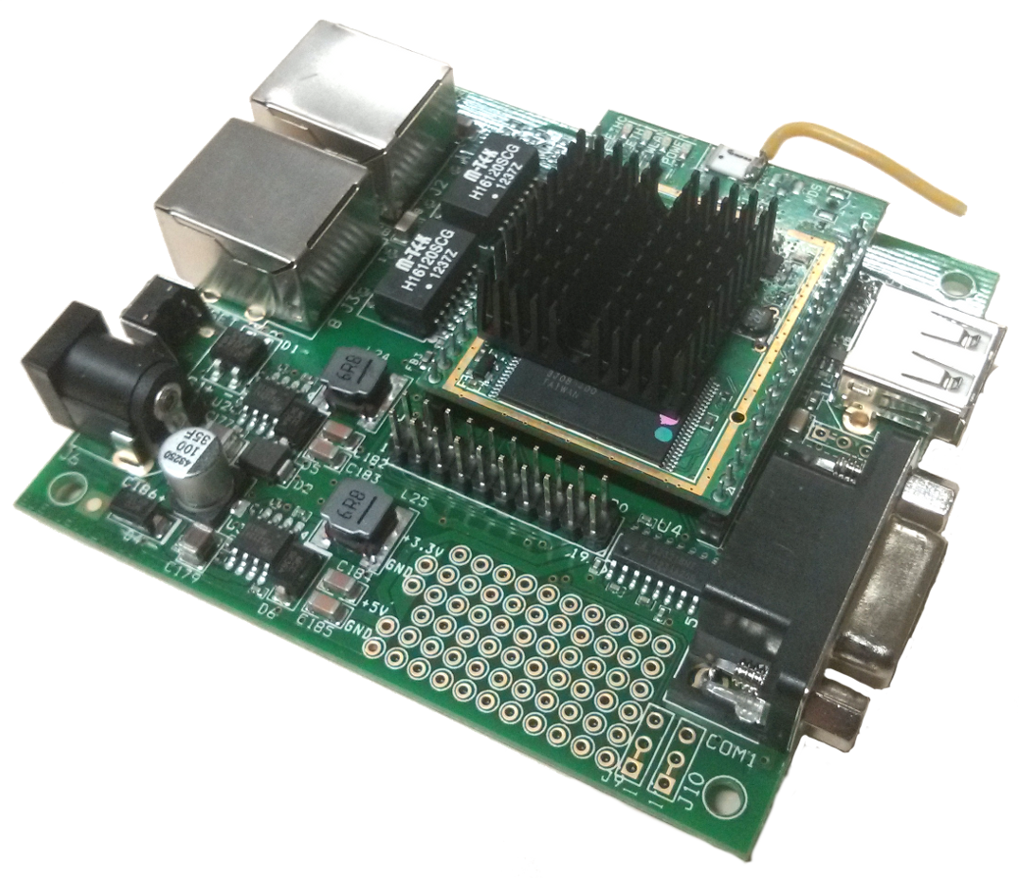
\includegraphics[width=7cm]{carambola.png}\\
\caption{Fotografie des Carambolas}{}
\end{figure}

Das Entwicklungsboard \textbf{Carambola}\cite{CARAM1} wird von der der Firma UAB
"`8devices"' hergestellt und besteht aus einer kleinen Platine mit einem Ralink
RT3050\cite{RA01} Mikrocontroller(MIPS-Architektur).

Der Mikrocontroller besitzt folgende Funktionen: 
\begin{itemize}
  \item Ralink RT3050 \SI{320}{\mega\hertz} MIPS SoC
  \item 5-Port Ethernetswitch
  \item 802.11n \SI{2,4}{\giga\hertz} WLAN
  \item I$^2$C, \gls{spi}, \gls{uart}
\end{itemize}
4 LEDs, eine WLAN-Antenne und ein \SI{32}{\mega\byte} Flash-Baustein sind dabei
bereits auf das Board integriert, die restlichen Anschlüsse sind über eine
Steckerleiste verfügbar.

Zusätzlich bietet "`8devices"' ein Entwicklungsboard an, auf das sich das
Carambola direkt aufstecken lässt. So können viele der vom Mikrocontroler
gebotenen Anschlüsse direkt verwendet werden. Das Entwicklungsboard besitzt
unter anderem zwei Ethernet-Anschlüsse, einen RS232-Anschluss, einen
USB-Anschluss und einen kleinen Bereich für eigene Elektronik\-aufbauten.

Das Carambola wird mit \textbf{OpenWRT}, einem linuxbasierten
Betriebssystem für eingebettete Geräte, betrieben. Dieses wird in
\autoref{subs:owrt} näher beschrieben.

Da das Carambola eine MIPS-Architektur besitzt, muss ein Cross-Compiler
eingesetzt werden, um Software für das Carambola erstellen zu können.
\begin{definition}[Cross-Compiler]
Ein Cross-Compiler ist ein spezieller Compiler, der den Quellcode einer
Software für eine andere als die ausführende Architektur kompilieren kann. Er
kommt dann zum Einsatz, wenn es nicht praktikabel oder schlicht unmöglich ist,
die Anwendung auf dem Zielsystem zu kompilieren. Dies kann zum Beispiel dann der
Fall sein, wenn ein eingebettetes System über nicht ausreichend Ressourcen
(Speicherplatz) verfügt, um den Kompilationsvorgang durchzuführen.
\end{definition}

\subsection{Zielsystem}
Das zu entwerfende Entwicklungssystem sollte ein möglichst
großes Spektrum potentieller Architekturen und Funksysteme abdecken können, so
dass es später einfach ist, das exemplarisch zu entwickelnde Zielsystem durch
ein anderes zu ersetzen. Dies sollte sich in einer möglichst
\textbf{generischen} Wahl der Komponenten eines beispielhaften Zielsystems
widerspiegeln.

Da Mikroprozessoren mit \textbf{ARM-Architektur} einen Anteil von rund
71\%\cite{IDC01} an allen verkauften CPUs haben, scheint es beinahe
selbstverständlich, sich für eine solche CPU zu entscheiden.

Bedingt durch die hohe Verbreitung von ARM Rechenkernen existiert allerdings
auch eine große Anzahl an Entwicklungsboards, die in Frage kommen.

Dabei ist es wichtig, eine Entscheidung eher nach Kriterien der Energieeffizienz
als der Rechenleistung zu treffen, da das Zielsystem später stark integriert
und unter Umständen auch unabhängig von einer Stromversorgung arbeiten können
soll.

Wählt man einen ARM-Kern nach der Energieeffizienz aus, fällt einem hierbei die
Reihe der Cortex-M Prozessoren auf. Sie liegen mit ihrem geringen Energiebedarf
in einem Bereich, der z.B. für Batteriebetrieb sehr gut geeignet ist. Aus diesem
Grund optimieren viele Chiphersteller, die Cortex-M Kerne verbauen, diese genau
dafür.

\begin{figure}[!ht]
\centering
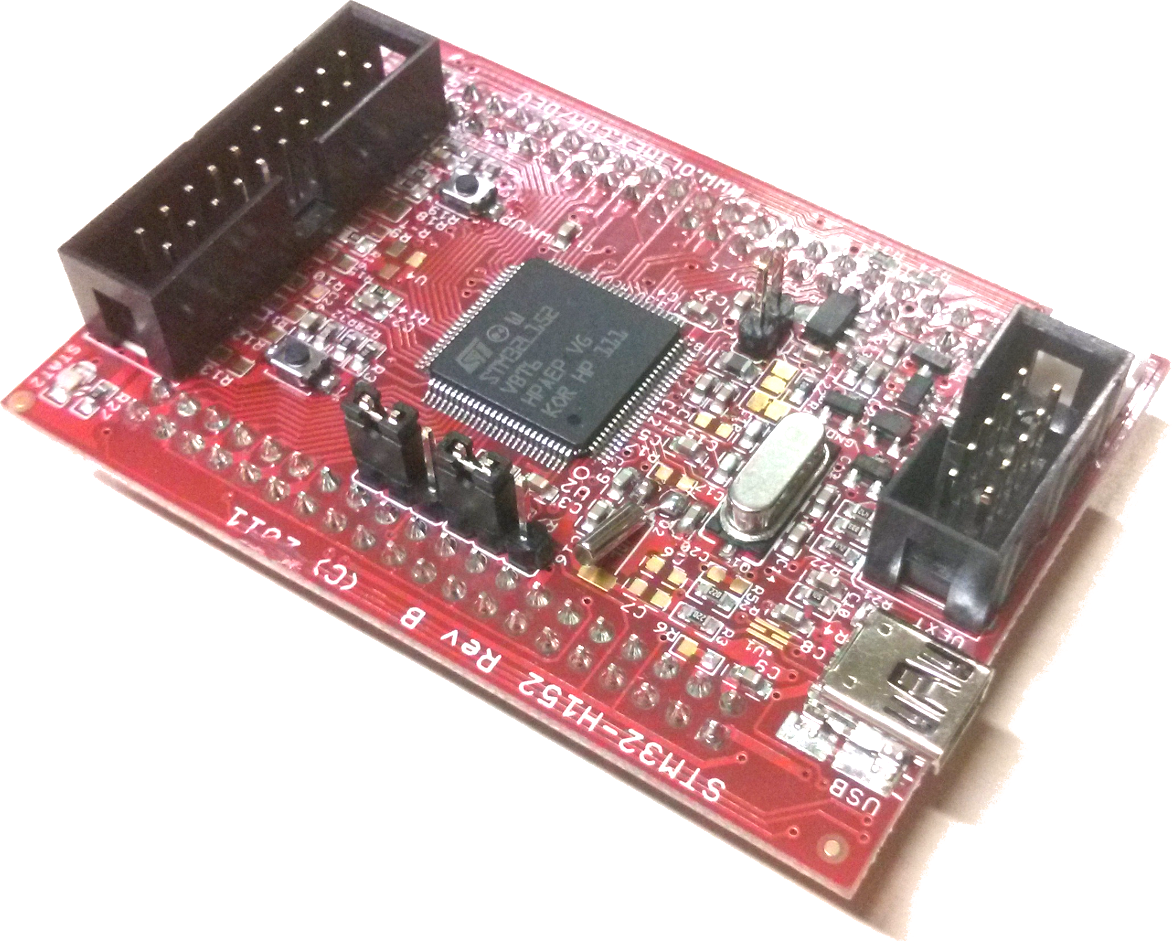
\includegraphics[width=7cm]{stm32.png}\\
\caption{Fotografie des STM32-H152}{}
\end{figure}

Das Entwicklungsboard "`STM32-H152"'\cite{OLI2} des Herstellers
\emph{Olimex Ltd.} besitzt mit dem \\STM32L152VBT6 der Firma
\emph{STMicroelectronics} genau einen solchen
energieeffizienten ARM-Mikrocontroller.

Auch das Board ist speziell auf den Batteriebetrieb ausgelegt und besitzt neben
einem USB-Anschluss für Stromversorgung und Datenübertragung eine 20-polige Buchse zum
Anschluss eines \gls{jtag}-Debuggers und einen Schaltkreis zum Laden von
Lithium-Ionen/Lithium-Polymer Batterien.

Außerdem befindet sich auf dem Board ein, bei \emph{Olimex}-Produkten häufig
eingesetzter, 10-poliger Anschluss. Für diesen "`UEXT"' getauften Anschluss
bietet \emph{Olimex} eine Reihe von Erweiterungsboards an, die sich so einfach
verbinden lassen. Dabei spezifiziert Olimex lediglich die Zuordnung
verschiedener Pins zu Funktionen, die auf den meisten Mikrocontroller
vorhanden sind(\gls{spi}, I$^2$C und \gls{uart}).

\subsection{Funkmodul} Die auf dem Markt verfügbaren Funkmodule lassen
sich grundsätzlich in zwei Kategorien einteilen.

Jedes Funkmodul besteht mindestens aus einem \textbf{Transceiver}. Dieser
Transceiver umfasst zumindest die analogen Komponenten der physikalischen
Schicht wie Analog-Digital-Wandler, Digital-Analog-Wandler, Filter, Verstärker,
Frequenzerzeuger. Je nach Ausführung werden, ahängig davon ob der Transceiver
für ein spezifisches Protokoll eingesetzt werden soll, auch die Bauteile des
Medium-Access-Layers (Checksummenprüfung, Buffer, Kollisionsvermeidung) in
einen Transceiver integriert.

Für viele Funkprotokolle stehen jedoch auch \textbf{Single-Chip Solutions}
zur Verfügung. Diese Bauteile bestehen sowohl aus einem Transceiver als auch,
neben anderen Bauteilen, aus einem eigenen Mikrocontroller. Dieser übernimmt die
Aufgaben höherer Netzwerkschichten und wird dafür oft über einfache Protokolle
wie \gls{uart} oder \gls{spi} angesprochen.

Dies bedeutet jedoch gleichzeitig mehr Hardware, da ein integrierter
Mikroprozessor betrieben werden muss und somit Strom benötigt.
Außerdem verhindert die hohe Abstraktion der Kommunikation genauere Einblicke in
deren Abläufe.

\begin{figure}[!ht]
\centering
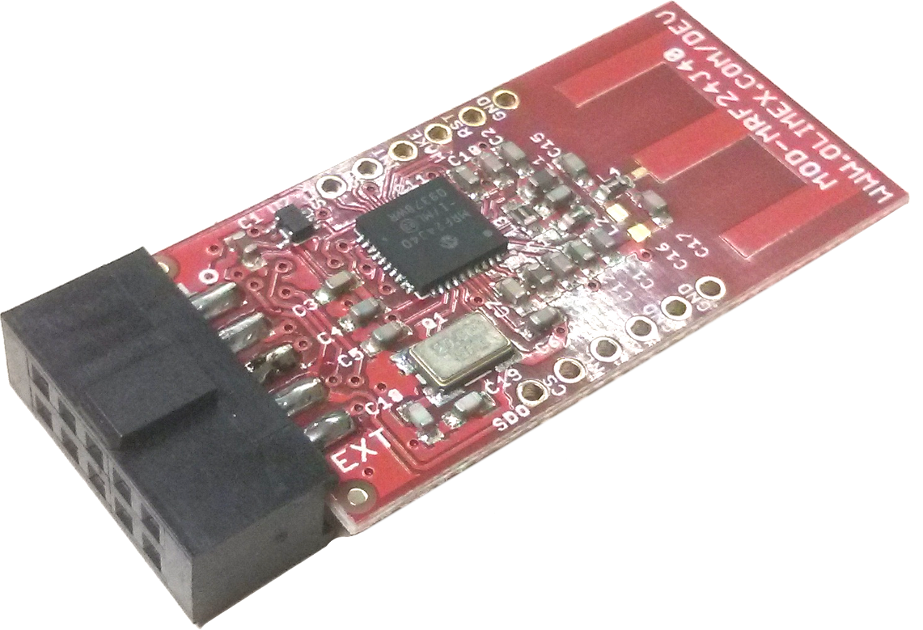
\includegraphics[width=4cm]{mrf24.png}\\
\caption{Fotografie des MRF24J40}{}
\end{figure}

Da es jedoch auch möglich sein soll, die Abläufe des Funkprotokolls erfassen ud
visualisieren zu können, sollte der Chip nicht zu abstrahiert funktionieren. Die
Wahl muss also zwangsläufig auf einen \textbf{Transceiver} fallen.

Da, wie zuvor erwähnt, eine Vielzahl verschiedenster Module für den "`UEXT"'
Anschluss existieren, gibt es hierfür auch ein Modul mit einem Transceiver.

Das Modul "`MOD-MRF24J40"' verwendet den Chip MRF24J40\cite{MRF} der Firma
Microchip Technology Inc. Der Chip ist eine IEEE 802.15.4\cite{IEEE01}
kompatible Realisierung eines Funktransceivers und implementiert die im Standard
spezifizierten PHY- und \gls{mac}-Layer.

Das Modul enthält eine integrierte Antenne und stellt die vom Chip zur
Datenkommunikation genutzte \gls{spi}-Schnittstelle über den "`UEXT"'-Stecker
zur Verfügung.
\section{Debugging}
\subsection{Schnittstellen}
Das Debugging eines eingebetteten Systems erfordert meist eine kombinierte Hard-
und Softwarelösung.

Der Softwareteil ist oft in die \gls{ide} des Entwicklers eingebunden oder lässt
sich zumindest vom Arbeitsplatz des Entwicklers aus steuern. Die Befehle des
Entwicklers (Setzen eines Breakpoints, Abfrage von Registerwerten, etc.) werden
vom Softwaretreiber anschließend in Steuerbefehle des Hardwarebauteils
umgesetzt. Das Hardwaremodul übernimmt hierauf, unter Nutzung eine
standardisierten Schnittstelle, die Kommunikation mit dem Zielsystem.

Als \emph{Schnittstellen} sind für diese Zwecke vor allem \gls{jtag} und
\gls{swd} verbreitet. Während \gls{jtag} ursprünglich primär zum Testen von Bauteilen
konzipiert wurde, erweitert \gls{swd} dieses Konzept um speziell für das
Debuggen nützliche Funktionen (Tracing, Paritätschecks) und reduziert die Anzahl
zwingend notwendiger Pins von 4 auf 2. Da \gls{swd} aber von
ARM speziell für Prozessoren mit eingebautem \emph{CoreSight}-Modul entwickelt
wurde, ist Unterstützung hierfür nicht auf allen ARM-Controllern anzutreffen. \gls{jtag}
hat hier eine wesentlich größere Verbreitung und wird auch
architekturübergreifend genutzt. Die \textbf{Wahl von \gls{jtag}} würde eine
spätere Erweiterung auf andere Architekturen somit erleichtern.
\subsection{OpenOCD - Open On-Chip Debugger}
Betrachtet man die Möglichkeiten zum Debuggen von ARM-Mikrocontrollern via
\gls{jtag} unter einem Linuxsystem, landet man beinahe zwangsläufig beim Open
Source Projekt \textbf{OpenOCD}. Dieses Projekt ist im Rahmen einer
Diplomarbeit\cite{OOCD2} an der \emph{FH Augsburg} entstanden und hatte die
Entwicklung einer quelloffenen Software zum Debuggen von ARM-Mikrocontrollern zum Ziel.
\emph{OpenOCD} fungiert dabei als Schnittstelle zwischen einem \gls{jtag}-Debugger und
einer Benutzeroberfläche.

\emph{OpenOCD} ist hochgradig modular gehalten und unterstützt daher eine große
Bandbreite von \gls{jtag}-Adaptern, verschiedenste Mikrocontroller und
Architekturen (unter anderem \emph{ARMv7}, \emph{ARMv4}, \emph{AVR32},
\emph{MIPS}), einige Echtzeitbetriebssysteme(\emph{FreeRTOS}, \emph{ChibiOS},
\emph{ThreadX}) und diverse Flash-Speicher.

Die Konfiguration von \emph{OpenOCD} erfolgt dabei über simple Skripte, die vom
Hauptprogramm beim Start eingelesen werden.

Auch der auf dem Olimex-Board verwendete Mikrocontroller "`STM32L152VB"' wird
von \emph{OpenOCD} als "`STM32L"' unterstützt.

\emph{OpenOCD} lässt sich dabei entweder über eine eigene Benutzeroberfläche via
Telnet-Protokoll oder mittels eines \gls{gdb}-Clients bedienen.

\begin{definition}[GDB]
Der \gls{gdb} ist der Standard-Debugger unter
Unix-Betriebssystemen. Er bietet unter Anderem die Möglichkeit, ein Programm im
laufenden Betrieb anzuhalten, Breakpoints zu setzen oder Single-Stepping
durchzuführen. Der \gls{gdb} besitzt keine grafische Oberfläche, sondern
lässt sich über eine Kommandozeile bedienen. Er bietet die Möglichkeit, von
einem Client über TCP/IP ferngesteuert zu werden. 
\end{definition}

Der entscheidende Punkt hierbei ist, dass \gls{gdb}(und auch \emph{OpenOCD})
grundsätzlich einen "`Remote"'-Modus anbietet. Dies wird dadurch möglich, dass
\gls{gdb} in einen "`Server"' und einen "`Client"' unterteilt ist. Dabei
übernimmt der "`Server"' die Kontrolle des Zielsystems oder der Zielsoftware,
wird aber gleichzeitig selbst vom \gls{gdb}-"`Client"' gesteuert. Der Entwickler
bedient dann den Client und damit nur indirekt den Debugger selbst.

Verwendet man \gls{gdb} im "`Remote"'-Modus, kann diese Steuerung über einen
beliebigen TCP-Port und damit auch über das Netzwerk erfolgen.

Setzt man \emph{OpenOCD} nun also auf dem Carambola ein, lässt sich diese Trennung
ausnutzen, um ein Debugging über eine beliebige Netzwerkverbindung zu
realisieren.
\subsection{OpenWRT}\label{subs:owrt}
OpenWRT ist ein ursprünglich aus dem von Linksys zur Verfügung
gestellten Quellcode des Routers "`WRT54G"' \cite{OWRT} hervorgegangenes
Opensource Projekt.

Ziel dieses Projektes ist die Entwicklung eines Betriebsystems, das sich
über ein Paketverwaltungssystem beliebig anpassen und dessen Dateisystem sich
beliebig beschreiben lässt. Dies soll es dem Nutzer ermöglichen, das System von
nicht benötigten Funktionen zu befreien, beziehungsweise auf seine Bedürfnisse
zuzuschneiden. Aus diesem Grund verfügt \emph{OpenWRT} über eine große Anzahl
für dieses System bereits portierter Bibliotheken und Anwendungen.

OpenWRT wird hauptsächlich als Firmware auf Routern verschiedenster Hersteller
angeboten. Es zeichnet sich durch eine hohe Konfigurierbarkeit bei
gleichzeitiger Unterstützung verschiedenster Plattformen aus. So werden neben
MIPS zum Beispiel noch ARM, PowerPC und x86 unterstützt. 

 \subsubsection*{Paketverwaltung
und Kompiliervorgang} \emph{OpenWRT} besitzt mit \textbf{opkg} ein Tool zur Paketverwaltung von
Anwendungen.
Hierbei kann die Software in Form von *.ipk-Files aus "`Repositories"'
installiert werden. Durch dieses Tool wird es möglich, das eingebettete System
für die eigenen Bedürfnisse anzupassen.
\begin{definition}[Repository]
Ein \emph{Repository} enthält kompilierte Anwendungen für ein bestimmtes
Betriebssystem und eine spezifische Architektur. Über eine
Paketverwaltungssoftware kann auf das Repository zugegriffen, Software
heruntergeladen und installiert werden. Abhängigkeiten gegenüber anderen
Softwarepaketen werden meist selbstständig erkannt und zusätzlich installiert.
\end{definition}
Die Erstellung neuer Pakete für OpenWRT wird durch stark modifizierte Makefiles
wesentlich vereinfacht.
 \begin{definition}[Makefile]
Ein \emph{Makefile} ist eine Datei, die Steuerbefehle für das Tool
\texttt{make} enthält. \texttt{make} wird überwiegend eingesetzt, um Quellcode
in ausführbare Programme und Bibliotheken zu übersetzen. Durch seinen hohen
Grad an Abstraktion können \emph{Makefiles} jedoch auch für andere Aufgaben
"`zweckentfremdet"' werden.
\end{definition}

%%\begin{minipage}[c]{\textwidth}
\emph{OpenWRT} liefert alle nötigen Bestandteile mit, um ein vollständiges Image
für das eingebettete System zu erstellen.
Der Ablauf ist dabei wie folgt:
\begin{itemize}
  \item Mittels des Befehls \listinlsh{make menuconfig} lässt sich der folgende
  Kompiliervorgang in einer grafischen Oberfläche anpassen. Dazu zählen die zu
  erstellenden Anwendungen, Konfigurationsparameter des Kernels und
  Voreinstellungen der Anwendungen.
  \item Durch das Eingeben von \listinlsh{make} wird der Kompiliervorgang
  gestartet
  \item Der Quellcode der Toolchain wird heruntergeladen und kompiliert
  \item Der Quellcode des Basissystems wird heruntergeladen und kompiliert
  \item Die einzelnen Pakete werden erstellt:
  \begin{itemize}
    \item Herunterladen des Quellcodes
    \item Anwenden von nötigen OpenWRT-Patches
    \item Kompilieren der Anwendung
    \item Erstellen der *.ipk-Datei
  \end{itemize}
\end{itemize}
%%\end{minipage}

Soll \emph{OpenOCD} nun auf diese Plattform portiert werden, ist es wünschenswert,
das Programm direkt in diesen Prozess des Paketverwaltungssystems einzubinden.
Hierfür muss ein geeignetes \emph{Makefile} erstellt werden.

Diese hohe Abstraktion hat gleichzeitig den Vorteil, dass statt des Carambolas
jede beliebige Plattform verwendet werden kann, die von OpenWRT unterstützt
wird.

\subsection{Wahl eines JTAG-Adapters}
\emph{OpenOCD} unterstützt eine große Anzahl verschiedener \emph{\gls{jtag}-Adapter}.
Viele dieser Adapter haben dabei jedoch im Grunde ähnliche Komponenten verbaut.

Neben den industriellen Lösungen mit speziell entwickelten Bauteilen(Segger
J-Link\cite{SEG}, ST Micro ST-Link\cite{STM01}), existieren auch viele
Alternativen, die bereits existierende Bauteile verwenden. So kommt zum Beispiel oft der
\emph{FT2232}-Chip zum Einsatz, der auf die Umsetzung von USB-Daten zu einem
seriellen bzw. parallelen Ausgang spezialisiert ist. Neben kommerziellen
Adaptern (Amontec JTAGkey2\cite{AMO}, Olimex ARM-USB-TINY-H\cite{OLI})
existieren auch einige Open Source Lösungen, in denen der \emph{FT2232} zum
Einsatz kommt (OOCDLink\cite{OCDL}, Turtelizer 2\cite{TURT}). Eine Auflistung
aller mit \emph{OpenOCD} kompatiblen Adapter findet sich in dessen "`User Guide"'\cite{OOCD}.

Entscheidend für die Wahl eines Adapters sollte zum einen die Anzahl der
unterstützten Zielsysteme sein. Diese definiert sich hauptsächlich über die
vom Adapter unterstützte \textbf{Spannung}. Da viele Mikrocontroller mit
$\SI{3.3}{\volt}$ oder $\SI{5.5}{\volt}$ betrieben werden, sollte der Adapter
zumindest diese beiden Spannungen unterstützen. Je größer diese Spanne jedoch ist, desto flexibler kann
er später eingesetzt werden.

Auch unterscheiden die Adapter sich im Vorhandensein von \textbf{adaptivem
Clocking}. Diese Funktion erlaubt es dem Adapter, sich an die aktuelle
Taktfrequenz des Zielsystems anzupassen. Da viele Mikrocontroller direkt nach
dem Start oder in einem Deep-Sleep-Zustand mit einer geringen Taktzahl arbeiten
und die aktuelle Taktzahl des Zielsystems oftmals die maximal mögliche
\gls{jtag}-Taktzahl vorgibt, müsste der Adapter anderenfalls unter Umständen langsamer
laufen. \emph{Adaptives Clocking} erlaubt es dem Zielsystem, eine Art
"`Rückmeldung"' über die, aktuell gültige, maximale \gls{jtag}-Taktzahl zu geben.

Im Rahmen dieser Arbeit soll der \textbf{ARM-USB-TINY-H} von Olimex zum Einsatz
kommen.
Dieser Adapter besitzt einen der verbreiteten \emph{FT2232}-Chips, bietet
Adaptives Clocking und unterstützt einen Spannungsbereich von $\SI{2.0}{\volt}$
bis $\SI{5.0}{\volt}$.

\subsection{Zielsetzung}
%%\begin{minipage}[c]{\textwidth}
Folgende Punkte sollen im Rahmen dieser Arbeit für ein funktionierendes
Debugsystem umgesetzt werden:
\begin{itemize}
  \item OpenWRT muss \textbf{kompiliert} und konfiguriert werden werden.
  \item Für \emph{OpenOCD} muss ein \textbf{Makefile} erstellt werden, mithilfe
  dessen über den \\(Cross-)Kompiliervorgang eine Paketdatei für
  OpenWRT erstellt wird.
  \item \emph{OpenOCD} muss so \textbf{(vor-)konfiguriert} werden, dass sich das
  Zielsystem damit debuggen lässt.
  \item Eine \textbf{\gls{ide}} muss so eingerichtet werden, dass sie \emph{OpenOCD}
  über \gls{gdb} als entfernete Debugging-Schnittstelle verwendet.
\end{itemize}
%%\end{minipage}
\section{Datenanalyse}\label{sec:datenan}
Ein weiterer wichtiger Bestandteil dieses Entwicklungssystems ist die
\emph{Analyse} von Daten, die das Zielsystem erzeugt. Da das Zielsystem über
eine Funkschnittstelle verfügt, muss die für das Zielsystem zu entwickelnde
Software diese Schnittstelle sicher auch in Betrieb nehmen können.
\subsection{Anforderungen}
Aufgabe dieses Teils des Entwicklungssystems wird es sein, die Erfassung der in
\autoref{sect:szenarien} erwähnten Szenarien zu erleichtern.

Bedingung für die Erfassung von Daten seitens des Entwicklungssystems ist, dass
das Zielsystem diese Daten überhaupt in einer erfassbaren Form zur Verfügung
stellt. Hierbei muss jedoch beachtet werden, dass nicht jedes Zielsystem über
alle Anschlussmöglichkeiten verfügen kann.

Um die Daten vom Zielsystem zu erfassen, bietet sich zum Beispiel die Nutzung
des \textbf{\gls{uart}} an. Hierfür muss jedoch die Software des Zielsystems so
angepasst werden, dass es die zu sammelnden Daten über \gls{uart} ausgibt.

\begin{definition}[UART]
\glsreset{uart}Der \gls{uart} ist eine, in Mikrocontrollern sehr weit
verbreitete, elektronische Schaltung zur seriellen Übertragung von Daten. In
seiner Minimalkonfiguration benötigt der \gls{uart} nur zwei Pins (RX ---
Receive, TX --- Transmit), da, durch Festlegung auf einen gemeinsamen Takt, auf
ein Taktsignal verzichtet werden kann. Dies ermöglicht eine Nutzung von
\gls{uart} auch in einem stark integriertem Zielsystem.
\end{definition}

Um die Daten später sortieren und analysieren zu können, müssen vom
Entwicklungssystem mindestens folgende Daten erfasst werden.
\begin{itemize}
  \item Vom Zielsystem \textbf{ausgegebene Daten}
  \item \textbf{Zeitpunkt} der Erfassung der Daten
\end{itemize}

Besonderes Augenmerk muss hierbei auf die Synchronizität der einzelnen Module
des Entwicklungssystems gelegt werden. Auf diesen Umstand wird in
\autoref{subs:time} weiter eingegangen. 

\subsection{Erforderliche Präzision}\label{subs:praezision}
Für viele Vorgänge der Funkschnittstelle ist eine gewisse Genauigkeit wichtig.
Diese drückt sich insbesondere in der Genauigkeit der vom Entwicklungssystem
verwendeten Zeitstempel aus.

Eine Möglichkeit die erforderliche Präzision analysieren zu können ist die
Untersuchen des Kollisionsvermeidungs-Algorithmus'.

Hierfür setzt der, in unserem Funkmodul verwendete, 802.15.4 Standard in seinem
\gls{mac}-Layer zum Beispiel CSMA/CA ein\cite{IEEE01}.
\begin{definition}[CSMA/CA]
\emph{CSMA/CA} ist ein Algorithmus zur Kollisionsvermeidung innerhalb eines
Netzwerks. Hierbei prüft der Sender vor dem eigentlichen Sendevorgang über
einen definierten Zeitraum, ob das Übertragungsmedium (zum Beispiel Funk oder
Kabel) "`frei"' ist. Wird das Medium bereits verwendet, wartet der der Sender
eine zufällige Zeitperiode (Back-off Periode) und überprüft den Zustand erneut.
Sobald der Sendekanal "`frei"' ist, beginnt der Sendevorgang. Der Empfang der Daten muss
von der Gegenstation mittels \texttt{ACK} bestätigt werden.
\end{definition}
Da \emph{CSMA/CA} jedoch im \gls{mac}-Layer stattfindet und dieser bereits
in das gewählte Funkmodul integriert ist, wird es vermutlich schwierig,
die Daten aus dem Modul selbst zu beziehen. Hier könnte man sich durch
die Analyse der empfangenen Daten behelfen.

Durch das integrierte \emph{CSMA/CA} lässt sich zwar der Versandzeitpunkt nicht
exakt bestimmen, jedoch aber der Empfangszeitpunkt. Untersucht man nun die
Differenz zwischen Sende- und Empfangsvorgang, lässt sich unter Umständen
erkennen, ob ein Backoff und damit eine erfolgreiche Kollisionsvermeidung
erfolgt ist.

Folgende Rechnung nach\cite{JENN} erläutert die Dauer einer Backoff-Periode.

\begin{align}\label{calc:init}
\mathit{InitialbackoffPeriod} &=(2^{BE}-1)*\mathit{aUnitBackoffPeriod} \\
&=(2^3-1)*\SI{320}{\micro\second}\nonumber \\
&= \SI{2240}{\micro\second} = \SI{2,24}{\milli\second} \nonumber 
\end{align}

Vor jedem Sendevorgang wird nach Spezifikation des \emph{CSMA/CA} ein zufälliger
Zeitraum \emph{InitialbackoffPeriod} gewartet. Erst anschließend wird der Kanal
auf Belegung überprüft. Diese \emph{InitialbackoffPeriod} berechnet sich nach
\autoref{calc:init}. 

Zu dieser Backoff-Periode kommt die anschließende Prüfung auf Belegung
(\gls{cca}) mit einer Dauer von 8 Symbol-Perioden (\SI{128}{\micro\second}). 

Im \SI{2,4}{\giga\hertz}-Band besteht ein Symbol aus 4 Bit. Eine Symbol-Periode
benötigt also, bei einer Übertragungsgeschwindigkeit von
\SI{250}{\kilo\bit\per\second}, eine Dauer von \SI{16}{\micro\second}.
($\frac{\SI{4}{\bit}}{\SI{250}{\kilo\bit\per\second}}=\SI{16}{\micro\second}$)

\emph{aUnitBackoffPeriod} ist in der Spezifikation mit 20 Symbol-Perioden also
\SI{320}{\micro\second} definiert. Zu Beginn ist \emph{BE}, der
Backoff-Exponent, standardmäßig auf 3 eingestellt. Dieser Zähler erhöht sich
jedoch mit jedem Mal, den ein \gls{cca} fehlschlägt.

Selbst für einen erfolgreichen Sendevorgang vergehen also bereits bis zu
\SI{2,24}{\milli\second}. Schlägt das \gls{cca} fehl, wird die
\autoref{calc:init} mit einem um 1 erhöhten \emph{BE} wiederholt und erneut
gewartet. Hierdurch kann ein Datenpaket in der von der IEEE vorgegebenen
Standardkonfiguration um bis zu \SI{9,92}{\milli\second} pro \gls{cca}-Versuch
verspätet werden ($(2^5-1)*\SI{320}{\micro\second = \SI{9920}{\micro\second}}$
mit einem maximalen \emph{BE} von 5).

\begin{figure}[!ht]
\centering
\begin{sequencediagram}
\setthreadbias{center}
\newthread[0]{node1}{Knoten 1}
\newthread[2]{node2}{Knoten 2}
\newthread[2]{node3}{Knoten 3}
\mess[2]{node1}{Anfrage 1}{node2}
\node[anchor=east,inner sep=10pt] (t0) at (mess from) {$t_0$};
\prelevel{2}
\mess[1]{node3}{Anfrage 2}{node2}
\node[anchor=west,inner sep=10pt] (t1) at (mess from) {$t_1$};
\node[anchor=north west,inner sep=10pt] (t2) at (mess to) {$t_2$};
\node[cross out,draw,minimum size = 18pt,very thick] at ($(mess from)!0.5!(mess
to)$) {};
\begin{callself}[5]{node3}{random\_backoff()}{}
\end{callself}
\mess[1]{node3}{Anfrage 2}{node2}
\node[anchor=east,inner sep=10pt] (t3) at (mess to) {$t_3$};
\end{sequencediagram}\\
\caption{Gleichzeitiger Sendevorgang mit Kollisionvermeidung}{Da Knoten 3 vor
seinem ersten Sendevorgang erkennt, dass bereits Daten übertragen werden, muss
er einen zufälligen Zeitraum warten, bevor ein Übertragungsversuch erfolgen
kann.}
\label{fig:kol}
\end{figure}

\autoref{fig:kol} visualisiert einen Sendevorgang mit einspringender
Kollisionsvermeidung. Zu Zeitpunkt $t_0$ beginnt \emph{Knoten
1} mit dem Senden von Daten. \emph{Knoten 3} führt bei $t_1$ ein \gls{cca}
durch und stellt fest, das bereits Daten gesendet werden. Seine Übertragung
wird also um eine Backoff-Periode zurückgestellt. \emph{Knoten 2} empfängt bei
$t_2$ die Daten von \emph{Knoten 1} und eine Weile später bei $t_3$ auch die
Übertragung von \emph{Knoten 3}. 

Da, wie zuvor erwähnt, das \gls{cca} auf Hardware-Ebene erfolgt, lässt sich der
tatsächliche Zeitpunkt des Absendens nicht herausfinden. Jedoch kann man anhand
der Differenz zwischen $t_0$ und $t_2$ erkennen, ob der ursprüngliche
Absendezeitpunkt $t_1$ von der \emph{Anfrage 2} dazwischen liegt. Auch könnte
man über die (vergleichbar große) Differenz zwischen $t_1$ und $t_3$ darauf
schließen, dass die Übertragung aufgrund eines fehlgeschlagenen \gls{cca}
verzögert wurde.

Will man diesen Ablauf zentralisiert erfassen, ergäbe sich im Optimalfall ein
Ablauf wie in \autoref{fig:kolmsg}. Zu Zeitpunkt $t_1$ würde \emph{Knoten 3}
anfänglich die Daten akzeptieren, jedoch hardwareseitig und durch ein
fehlgeschlagenes \gls{cca} noch nicht direkt absenden.

\begin{figure}[!ht]
\centering
\par\begin{tabu}{l c l}
Zielsystem & Zeitstempel & Nachricht\\
\hline
\emph{<Knoten 1>} & \emph{$t_0$} & Anfrage 1 gesendet\\ 
\emph{<Knoten 3>} & \emph{$t_1$} & Anfrage 2 gesendet\\
\emph{<Knoten 2>} & \emph{$t_2$} & Anfrage 1 erhalten\\
\emph{<Knoten 2>} & \emph{$t_3$} & Anfrage 2 erhalten\\
\hline
\end{tabu}\\
\caption{Erfassung der Daten des Ablaufs aus \autoref{fig:kol}}{Ein Ablauf
wie in \autoref{fig:kol} dargestellt, könnte diese Reihenfolge von
Nachrichten erzeugen.}
\label{fig:kolmsg}
\end{figure}

Bei einer minimal spezifizierten Größe des Payloads eines
IEEE 802.15.4-Paketes von \SI{2}{\byte}\cite{IEEE01} werden
\SI{672}{\micro\second} zur Übertragung benötigt. Dies zeigt
\autoref{calc:data}. Hierbei sind der \emph{overhead}-Anteil \SI{19}{\byte}
bestehend unter anderem aus Sequenznummer, Adressfeldern und Längenangabe aus
PHY- und \gls{mac}-Layer.
\begin{align}\label{calc:data}
\frac{(\SI{2}{\byte}+\mathit{overhead)*8}}{\SI{250}{\kilo\bit\per\second}}=\SI{672}{\micro\second}
\end{align}

Will man nun die erwähnten Abläufe sinnvoll erfassen, muss die Präzision der
Timer also bei \textbf{unter \SI{1}{\milli\second}} liegen. Erst diese
Genauigkeit würde ein sinnvolles Sortieren und Zuordnen der Abläufe ermöglichen.

\subsection{Bestandteile}\label{subs:best}
Der Teil des Entwicklungssystems, der für die Analyse der gesammelten Daten
zuständig ist, muss im Kern aus drei Teilen bestehen.
\begin{itemize}
  \item \textbf{Server} --- Läuft als Anwendung auf dem Carambola. Empfängt
  Daten über \gls{uart} und leitet diese an den Client weiter.
  \item \textbf{Client} --- Läuft auf dem System des Entwicklers. Verbindet sich
  zu der Serveranwendung und empfängt von ihr die gesammelten Daten.
  \item \textbf{Protokoll} --- Definiert die Kommunikation zwischen Server und
  Client.
\end{itemize}
Für die \emph{Clientanwendung} ist es von großer Bedeutung, dass sie sich zu
mehreren Serverinstanzen verbinden kann. Nur hierdurch wird es möglich, die
Daten von mehreren Zielsystemen erfassen und auswerten zu können.

Für die \emph{Serveranwendung} ist es nicht unbedingt notwendig aber
wünschenswert, mehrere verbundene \emph{Clients} verwalten zu können.
\subsection{Zeitsynchronisation}\label{subs:time}
Ein wichtiger Punkt im Entwurf dieses Systems ist die \textbf{Synchronisation
der Uhren} der jeweiligen Module. Nur so kann eine Vergleichbarkeit der
verarbeiteten Daten gewährleistet werden.

Aus \autoref{subs:praezision} ergibt sich, dass eine Präzision von mindestens
\SI{1}{\milli\second} gewährleistet werden sollte. Zu den nicht beeinflussbaren
Größen zählen hierbei zum Beispiel die für einen Kontextwechsel durch den
Scheduler des Betriebssystems nötige Zeit oder die Genauigkeit des
Systemquarzes.

Da der zu übertragene Zeitstempel die seit eines durch den Entwickler-Rechner
festgelegten Zeitpunktes vergangenen $\si{\micro\second}$ darstellt, muss diese
Zahl ausreichend groß dimensioniert sein. Eine 32-Bit Zahl reicht unter
Umständen für die Betrachtung längerer Zeitabstände nicht mehr aus
($2^{32}\si{\micro\second}\approx \SI{71}{\minute}$).

Eine \textbf{64-Bit} Zahl bleibt somit als einzige Möglichkeit. Sie bietet
ausreichend viel Platz ($2^{64}\si{\micro\second}\approx 584942~years$), um auch
über sehr große Zeiträume Daten aufzuzeichnen.

Ein erster Ansatz für den Synchronisationsvorgang wäre, bereits bestehende
Synchronisationstechniken wie \gls{ntp} zu verwenden. Diese haben jedoch den
Nachteil, dass sie für die Synchronisation immer eine aktive Verbindung zum
Internet oder einen lokalen \gls{ntp}-Server  benötigen. Außerdem sind, da
die Carambola-Systeme keine Echtzeituhren besitzen, Datum und Uhrzeit nach einem
Start des Systems auf die Unix Epoche gesetzt. Da \gls{ntp} direkt die
Systemzeit beeinflusst, würde dies unter Umständen Auswirkungen auf andere Prozesse
bedeuten.

Für die Zeitsynchronisation soll eine Abwandlung des Algorithmus von
Christian\cite{CHR} zum Einsatz kommen. Entscheidend ist hierbei, dass der
Synchronisationsvorgang vom Zeitgeber angestoßen wird. Dies erfordert eine
zusätzliche abschließende Datenübertragung.

Da TCP durch seine Flusskontrolle die Messung der Netzwerklatenz
durch eventuell Neuübertragungsversuche negativ beeinflussen kann, ist für die
Zeitsynchronisation die Verwendung von UDP nötig. Dies bedingt allerdings die
Verwendung einer Sequenznummer.

\begin{itemize}
  \item Der Client stößt den Synchronisationsvorgang an, indem er dem Server
  seinen aktuellen Zeitstempel $t_0$ mittels einer \texttt{PING}-Nachricht
  übermittelt.
  \item Bei Erhalt der Nachricht erfasst der Server seinen eigenen Zeitstempel
  als $t_1$.
  \item Anschließend bereitet er das Senden einer \texttt{PONG}-Nachricht als
  Antwort vor, erfasst einen weiteren Zeitstempel ($t_2$) und sendet die
  Nachricht.
  \item Bei Erhalt der Nachricht durch den Client, erfasst dieser seine eigene
  Zeit $t_3$ und übermittelt sie dem Server in einer, diesen
  Synchronisierungsprozess abschließenden, \texttt{STIM}-Nachricht.
\end{itemize} 
Dieser Vorgang ist in \autoref{fig:timeseq} visualisiert.

\begin{figure}
\centering
\begin{sequencediagram}[ht]
\newthread[0]{client}{:Client}
\newthread[3]{server}{:Server}
\mess[2]{client}{PING}{server}
\node[anchor=east,inner sep=10pt] (t0) at (mess from) {$t_0$};
\node[anchor=west,inner sep=4pt,label=above right:{$t_1$}] (t1) at (mess to)
{};
\mess[2]{server}{PONG}{client}
\node[anchor=west,inner sep=4pt,label=below right:{$t_2$}] (t2) at (mess from)
{}; \node[anchor=east,inner sep=10pt] (t3) at (mess to) {$t_3$};
\mess[2]{client}{STIM}{server}
\path (t0.east) |- coordinate(t01) (t1);
\draw[dashed] (t1) -- (t01);
\path (t3.east) |- coordinate(t23) (t2);
\draw[dashed] (t2) -- (t23);
\end{sequencediagram}
\caption{Ablauf der Zeitsynchronisation eines Servers}
\label{fig:timeseq}
\end{figure}

Nach Abschluss dieser Kommunikation lässt sich die Zeitdifferenz durch folgende
Formel errechnen.
\begin{equation}
\frac{t_1-t_0-t_3+t_2}{2}=\Delta t
\end{equation}
Um Abweichungen, zum Beispiel durch unterschiedliche Latenzen auf dem Hin- und
Rückweg im Netzwerk, auszugleichen, sollten mehrere dieser Vorgänge durchgeführt
und ein arithmetisches Mittel über die gesammelten Differenzen gebildet werden.
Dieser Mittelwert ist eine etwas bessere Annäherung an die tatsächliche
Differenz.

\subsection{Protokoll}
Insgesamt müssen für das Entwicklungssystem zwei \emph{Protokolle} spezifiziert
werden, da drei verschiedene Systeme eingesetzt werden.

\subsubsection*{Zielsystem --- Serveranwendung}
Für die Kommunikation zwischen dem Zielsystem und dem Carambola und damit der
Serveranwendung wird \gls{uart} als Schnittstelle eingesetzt.

\gls{uart} ist relativ flexibel in seiner Umsetzung. So lassen sich
diverse Paramter verändern (Baudrate, Stopbits, Paritätsbits). Dies
bedeutet jedoch auch gleichzeitig, dass es keine einheitliche Lösung geben kann.
Aus diesem Grund muss es möglich sein, diese Parameter unter Umständen an die
Bedürfnisse des Zielsystems anpassen zu können.

Eine hohe Flexibilität soll auch in der Art der übertragenen Daten
gewährleisten werden.

Es wird nur spezifiziert, dass über den \gls{uart}-Anschluss
gesendete Daten mit einem Zeilenumbruch enden müssen. Anschließend wird von der
Serveranwendung ein Zeitstempel generiert und die Daten im System
weitergereicht.

Dies erlaubt es dem Zielsystem, neben Debugausgaben des Funkmoduls auch
beliebige andere Nachrichten an das Entwicklersystem abzusetzen.

\subsubsection*{Serveranwendung --- Entwicklersystem}
Damit der Client und die Serveranwendungen über das Netzwerk kommunizieren
können, wird ein Protokoll zum Datenaustausch spezifiziert. Dieses Protokoll
legt sowohl den Aufbau der Datenpakete als auch die Abläufe der Kommunikation
fest.

Während die Übertragung der Nutzdaten (vom Zielsystem ausgegebene Daten) über
TCP erfolgt, läuft die Zeitsynchronisation über UDP ab. Die Verwendung von UDP
garantiert, dass keine Mehrfachübertragung eines fehlerhaften Datenpaketes
erfolgt, welche eine korrekte Zeitmessung verhindern würde.

Für die Übertragung der Nutzdaten ist aber zu entscheiden ob der Nagle
Algorithmus\cite{RFC896} deaktiviert werden muss, da die Daten ansonsten unter
Umständen zu stark verzögert werden.

Um das Protokoll erweiterbar zu halten, sollte es eine Möglichkeit geben, das
System später um andere Nutzdatentypen wie zum Beispiel Ausgaben einer \gls{spi} oder
I$^2$C-Schnittstelle erweitern zu können.

Das Protokoll soll folgende Funktionen erlauben:
\begin{itemize}
  \item \textbf{Zeitsynchronisation} wie in \autoref{subs:time} aufgeführt
  \item Übertragung von \textbf{\gls{uart}-Daten}
  \item \textbf{Erweiterungsmöglichkeit} für andere Datentypen
\end{itemize}

Jedes Datenpaket besteht dafür aus einem \textbf{Pakettyp}, der \textbf{Länge}
(Anzahl Byte) der Nutzdaten, einem \textbf{Zeitstempel} und optional den
\textbf{Nutzdaten} selbst. Die Übertragung erfolgt dabei, wie für die meisten
Netzwerkprotokolle üblich, in Big-Endian. Der Aufbau eines Datenpaketes ist in
\autoref{fig:bytefield} visualisiert.

\begin{figure}[h!]
\centering
\begin{bytefield}[bitheight=3.1ex,bitwidth=3em,endianness=big]{8}
\bitheader{0-7} \\
\begin{rightwordgroup}{Header}
\wordbox{1}{Type (1 Byte)} \\
\wordbox{2}{Length (2 Byte)} \\
\wordbox{8}{Timestamp (8 Byte)}
\end{rightwordgroup} \\
\wordbox[lrt]{1}{Data (n Byte)} \\
\skippedwords \\
\wordbox[lrb]{1}{}
\end{bytefield} \\
\caption{Systematischer Aufbau eines Datenpaketes}{Der Aufbau eines TCP-Paketes
ist mit dem eines UDP-Paketes identisch. Die Menge \emph{n} der Daten ist
auf 512 Byte beschränkt.}
\label{fig:bytefield}
\end{figure}

Die Größe des Headers beträgt 11 Byte und setzt sich wie folgt zusammen:\\
Für die Bestimmung des \textbf{Typs} eines Datenpaketes reichen 8 Bit. Dies
ermöglicht 256 verschiedene Pakettypen und somit ausreichend Spielraum für
potentielle Erweiterungen. Die Größe des \textbf{Zeitstempels} von 64 Bit ist in
\autoref{subs:time} erläutert worden. Die maximale Größe der an ein
Datenpaket anhängbaren Nutzdaten ist auf 512 Byte beschränkt. Dies erscheint
ausreichend groß für "`kurze"' Statusnachrichten. Hieraus ergibt sich, dass für
die Angabe der \textbf{Länge} 16 Bit benötigt werden.


Aus dem Ablauf in \autoref{subs:time} ist ersichtlich, dass bei den
UDP-Nachrichten einzig für \texttt{PING} und für \texttt{STIM} eine
Übermittlung des Zeitstempels wichtig ist, gleichzeitig allerdings auch eine
Sequenznummer benötigt wird. Verlagert man den zu übertragenden Zeitstempel der
\texttt{STIM}-Nachricht in den Bereich der \emph{Nutzdaten}, lässt sich das
\emph{Zeitstempel}-Feld im UDP-Ablauf durchgehend als Sequenznummer verwenden.
Die erste \texttt{PING}-Nachricht übermittelt somit indirekt auch die für den
weiteren Synchronisierungsablauf notwendige Sequenznummer in Form ihres eigenen
Zeitstempels.

In \autoref{fig:prot} sind die verschiedenen TCP- und UDP-Pakettypen aufgeführt. 
\begin{figure}[ht]
\centering
\begin{tabu}{l l l p{7cm}}
\multicolumn{3}{c}{\textbf{Server zu Client}}\\ \cline{1-3}
Protokoll & Abkürzung & Wert & Beschreibung \\ \hline
TCP & MESS & \texttt{0x01} & Allgemeine Nachricht des Servers. Eventuell als
Broadcast verursacht durch MESS von einem Client. \\
& UART & \texttt{0x02} & Der Server hat eine UART-Zeile empfangen. Die
empfangenen Daten sind als Payload angehängt. \\
& SPID & \texttt{0x03} & Der Server hat eine SPI-Zeile empfangen. Die
empfangenen Daten sind als Payload angehängt. \\
& PONG & \texttt{0x06} & Antwort des Servers auf TCP-PING vom Client. \\
UDP & PONG & \texttt{0x06} & Antwort des Servers auf PING vom Client.
Zeitstempel identisch mit PING.\\
\hline \\
\multicolumn{3}{c}{\textbf{Client zu Server}}\\ \cline{1-3}
Protokoll & Abkürzung & Wert & Beschreibung \\
\hline
TCP & MESS & \texttt{0x01} & Payload an alle verbundenen Clients senden.
(Broadcastfunktion)\\
& PING & \texttt{0x05} & Eine TCP-PONG-Antwort vom Server anfordern. Unabhängig
von der Zeitsynchronisation!\\
& EXIT & \texttt{0x10} & Den Server zum Schließen aller Verbindungen und Beenden
der Serveranwendung veranlassen. \\
UDP & PING & \texttt{0x05} &  Einen PING mit aktuellem Zeitstempel des Clients
senden.\\
& STIM & \texttt{0x04} & Letzter Schritt der Zeitsynchronisation. Den Zeitpunkt
des zuletzt erhaltenen \emph{PONG} als Payload anhängen. Zeitstempel identisch
mit PONG.\\
\hline \end{tabu}\\
\caption{Nachrichtentypen des Protokolls}{In dieser Tabelle ist mit
"`Client"' das Softwaremodul auf dem Entwickler-PC und als "`Server"' das
Gegenstück auf dem eingebetteten System gemeint. Die Spalte "`Wert"' enthält die
im Header als "`Typ"' bezeichnete Kodierung des Pakettyps.}
\label{fig:prot}
\end{figure}

\section{Deployment}
Die zum \emph{Debuggen} bereits bestehende \gls{jtag}-Verbindung lässt sich
ebenso verwenden, um Software auf das Zielsystem zu bringen.

Grundvoraussetzung ist hierfür jedoch, dass sich das \gls{rom} des Zielsystems
über den \gls{tap} erreichen lässt. Dies ist bei dem verwendeten ST Cortex M3
(und vielen anderen Mikrocontrollern) der Fall.
\subsection{Zielsetzung}
Es muss eine Möglichkeit gefunden werden, die Verwendung eines \gls{gdb}-Clients
zu automatisieren. Dadurch könnte man ein und dieselbe Firmware auf eine
beliebige Anzahl Zielsysteme verteilen.

Existiert diese Möglichkeit, kann der gleiche Weg genommen werden, um diese
Zielsysteme gesammelt resetten und somit in einen definierten Augangszustand
bringen zu können.
